%%%%%%%%%%%%%% 
% Fichero: EjTablas
% Autor: J. Salido (http://www.esi.uclm.es/www/jsalido)
% Fecha: febrero, 2017
% Descripción: Ejemplo básico de inclusión de tablas.
% Ejemplo del curso: “LaTeX esencial para preparación de TFG, Tesis
% y otros documentos académicos” (Esc. Sup. Informática-UCLM)
%%%%%%%%%%%%%%




%%%%%%%%%%%%%%
% Preámbulo del documento
%%%%%%%%%%%%%%
\documentclass[11pt,a4paper]{article} 
\usepackage[spanish,es-tabla,es-noindentfirst]{babel} % Opción para cambio de nombre
\usepackage[left=2cm,right=2cm,top=2cm,bottom=2cm]{geometry} % Márgenes 

% Tipografía
\usepackage{newpxtext}
\usepackage{newpxmath}

\usepackage{marvosym}
\usepackage{pifont} % Generación de símbolos especiales
\usepackage{textcomp}

\usepackage[T1]{fontenc} % Codificación de salida    
\usepackage{microtype} % Mejoras de microtipografía en la obtención de PDF (sólo para pdflatex)

\usepackage{siunitx} % Formateado de números y unidades en el SI.

% NOTA: Este paquete incluido más abajo produce -> LaTeX Error: Option clash for package xcolor
% Color
\usepackage[table,dvipsnames,svgnames]{xcolor}

% Generación de hiperenlaces
\usepackage[%
   pdftex,
   breaklinks,
   hidelinks=true,      % Oculta colores en los enlaces (negro)
    linktocpage=true,    % true = enlace al nº de pág., false=texto completo
%    colorlinks=true,         % true=colorea texto del enlace, false=recuadra el texto
	citecolor=red, % Color de la citas
	urlcolor=blue, % Color de las URL
	bookmarksnumbered=true % Incluye números en bookmarks
]{hyperref}
\usepackage{url}
\urlstyle{sf} % Estilo de URL sin serifas

% Listas
\usepackage{enumitem} % Mayor control de listas
\usepackage{multicol} % Elementos en varias columnas

% Gráficos
\usepackage{graphicx}  % Inclusión de figuras y escalado de cajas
\usepackage{float} % Control de posición de objetos flotantes y estilos
\usepackage[margin=10pt,labelfont=bf]{caption}

% Declaración del path donde están los archivos de figuras. 
% También se puede incluir el path en el nombre del fichero.
\graphicspath{{../figs/}}  
\DeclareGraphicsExtensions{.pdf,.png,.jpg}
% Lista de extensiones de ficheros por orden de precedencia. De este modo no hace falta indicar la extensión del fichero y en caso de existir dos fichero con el mismos nombre y extensión diferente se emplea el que tiene una extensión con mayor prioridad.

% Tablas
\captionsetup[table]{skip=5pt} 	% Separación del caption en las tablas aumentando el valor por defecto 

% Con estas instrucciones se ajustan los valores del índice
\setcounter{secnumdepth}{2} % Ajusta el valor del último nivel numerado
\setcounter{tocdepth}{2} %Ajusta el valor del último nivel que aparece en TOC


\author{Jesús Salido}
\title{Inclusión de tablas básicas en \LaTeX{}}
\date{\today}


%%%%%%%%%%%%%%
% Comienzo del documento
%%%%%%%%%%%%%%
\begin{document}
\maketitle
\begin{abstract}
	Explicación sencilla sobre cómo incluir y manejar tablas sencillas con \LaTeX{}.
\end{abstract}

\hrule
\tableofcontents
\listoftables
\bigskip
\hrule




\section{Tablas en \LaTeX{}}
La inclusión de tablas en documentos preparados con \LaTeX{} no es sencilla e incluso podría calificarse de <<engorrosa>>. Las tablas se crean con el entorno \texttt{tabular} en el que se indica el número de columnas y la alineación del texto en cada columna (l=izda., c=central, r=dcha.). Las líneas de separación en la tabla se indican mediante el carácter \texttt{`|'} (líneas verticales) o la macro \texttt{\textbackslash hline} (líneas horizontales). La separación del texto entre columnas se realiza con el carácter \texttt{`\&'} y la separación de filas con \texttt{`\textbackslash\textbackslash'}.

Para que la tabla sea manejada como un objeto \emph{float} debe incluirse en el entorno \texttt{table}, cuya ubicación se rige por los mismos principios que la inclusión de figuras o cualquier otro objeto flotante.

Un sitio muy apropiado para experimentar con las tablas y aprender los principios básicos de eso se proporciona en: \url{www.learnlatex.org/es/lesson-08}. En este sitio puedes encontrar una explicación sucinta de la creación de tablas en \LaTeX{} con numerosos ejemplos con los que practicar y que reproducimos en este documento.

Para obtener una interfaz mejorada de creación de entornos tabular en \LaTeX{} siempre se debe cargar el paquete \texttt{array}. En el ejemplo de la tabla~\ref{tab:simple} se muestra una tabla con un conjunto importante de propiedades como: líneas de separación (horizontales y verticales), distintos tipos de justificación, etc. Como puede comprobarse en dicho ejemplo, \LaTeX{} es capaz de realizar las tablas con multitud de elementos con una gran flexibilidad. Sin embargo, echando un vistazo al texto fuente podemos intuir que la elaboración de tablas es tediosa y tanto más cuanto mayor sea el tamaño y la complejidad de la tabla. Por supuesto, las tablas creadas en \LaTeX{} son armoniosas y congruentes con el texto general. Por ello, la inmensa mayoría de publicaciones científicas exigen que las tablas sean creadas de modo nativo mediante comandos \LaTeX{} y no se permite su inclusión como figura (p.~ej., de una captura de pantalla).

\begin{table}[H]%
	\centering
	\caption[Ejemplo de entorno \texttt{table}]{Tabla sencilla}		  \label{tab:simple}
    \begin{tabular}{l|l|l}
      \textbf{Animal}  & \textbf{Comida} & \textbf{Tamaño} \\
      \hline
      perro   & carne  & mediano \\
      caballo & heno   & grande  \\
      rana    & moscas & pequeño \\
    \end{tabular}
\end{table}

En el siguiente ejemplo se ha hecho uso de la macro \texttt{cline} para generar líneas que no abarcan todas las columnas de la tabla.

\begin{table}[H]%
	\centering
	\caption{Ejemplo de uso de la macro \texttt{cline}}
	\label{tab:cline}
	\begin{tabular}[t]{|r|l|}
	\hline
	7C0 & hexadecimal \\[1cm] % Ejemplo de separación fijada entre líneas
	3700 & octal \\ \cline{2-2}
	11111000000 & binario \\
	\hline \hline
	1984 & decimal \\
	\hline
	\end{tabular}
\end{table}

Hay que tener cuidado con la longitud del contenido de cada celda, ya que por defecto, \LaTeX{} no recorta el texto al tamaño de la línea. Para evitarlo se especifica el ancho de columna:

\begin{table}[H]%
	\centering
	\caption{Ejemplo de tabla con especificación de anchura de columna}
	\label{tab:anchura}
	\begin{tabular}{ | l | l | l | p{5cm} |}
	\hline
	Día & Temp Mín (\textdegree C) & Temp Máx (\textdegree C) & Previsión \\ \hline
	Lunes & 11 & 22 & Día claro y muy soleado. Sin embargo, la brisa de la tarde puede hacer que las temperaturas desciendan \\ \hline
	Martes & 9 & 19 & Nuboso con chubascos en muchas regiones. En Cataluña claro con posibilidad de bancos nubosos al norte de la región \\ 
    \hline
	\end{tabular}
\end{table}

Cuando las tablas tienen muchas columnas es posible hacer una declaración abreviada empleando la sintaxis \texttt{*\{num\}\{just\}} como en la tabla siguiente:

\begin{table}[H]%
	\centering
	\caption{Especificación abreviada en tabla}
	\label{tab:abreviada}
	\begin{tabular}{l*{6}{c}|r}
	Equipo            & J & G & P & E & F  & C & Pts \\
	\hline
	Manchester United & 6 & 4 & 0 & 2 & 10 & 5 & 12  \\
	Celtic            & 6 & 3 & 0 & 3 &  8 & 9 &  9  \\
	Benfica           & 6 & 2 & 1 & 3 &  7 & 8 &  7  \\
	FC Copenhagen     & 6 & 2 & 1 & 2 &  5 & 8 &  7  \\
	\end{tabular}
\end{table}







\section{Tablas incluidas como figuras}
Tal como muestran los ejemplos precedentes la preparación de tablas con \LaTeX{} es un proceso de cierta complejidad. Por el contrario las tablas, confeccionadas mediante hojas de cálculo, que puede incluirse en los documentos con los procesadores tipo \textsc{WYSIWYG} (\textsf{Word}, \textsf{OpenOffice}, etc.) siguen un proceso intuitivo y rápido. Existe un modo para aprovechar estas ventajas empleando \LaTeX{}. Para ello se puede salvar en formato \textsf{PDF} las tablas creadas con una hoja de cálculo (p.~ej.\ \textsf{Excel}) e incorporarlas en un documento \LaTeX{} mediante una tabla que sólo contiene una celda en la que incluimos el fichero gráfico con la tabla en formato \textsf{PDF}. 

La tabla~\ref{tab:figura} muestra un ejemplo de tabla creada con \textsf{Excel} e incluida como un fichero \textsf{PDF}. Este método permite emplear las tipografías disponibles en el sistema para las hojas de cálculo. Además, se pueden aplicar todas las opciones aplicables para los gráficos incluido el dimensionado de los mismos. Es importante señalar que si no se va a aplicar ningún escalado a la figura de la tabla, ésta debería crearse con el mismo tamaño de fuente que tendrá el texto normal del documento final y empleando preferiblemente una tipografía similar a la utilizada en el documento.

\begin{table}[H]%
	\centering
	\caption[Tabla \textsf{Excel}]{Ejemplo de tabla creada con \textsf{Excel} e incluida como figura}
	\label{tab:figura}
	\begin{tabular}{c}
%		\includegraphics{alimentos}
		\includegraphics{../figs/alimentos}
	\end{tabular}
\end{table}

Este método es aceptable para publicaciones como TFG y Tesis. Sin embargo, no es apropiado para publicaciones especializadas (p.~ej.\ revistas y congresos) y en estos casos la editorial suele rechazar el resultado por los estándares tan exigentes empleados. El problema deriva de que las fuentes empleadas por los programas externos emplean tipografías ligeramente diferentes a las empleadas por \LaTeX.
\end{document}
